\documentclass[tikz,border=2pt,11pt]{standalone}
\usetikzlibrary{arrows.meta}
\usetikzlibrary{positioning}
\usepackage{amsmath}
\usepackage{amssymb}
\usepackage{tikz}
\newcommand{\CPT}{\mathrm{CPT}}
\newcommand{\HF}{\mathrm{HF}}
\DeclareMathOperator{\Aut}{Aut}
\DeclareMathOperator{\FV}{FV}
\begin{document}
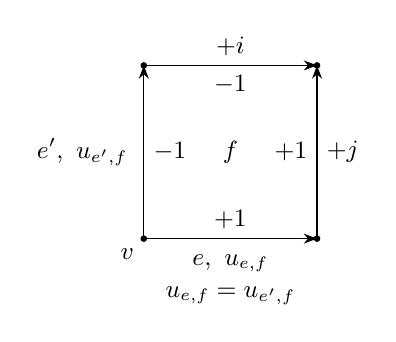
\begin{tikzpicture}[x=1cm,y=1cm,>=Stealth,font=\small]
  \draw[->] (0,0) -- (2.2,0);
  \draw[->] (2.2,0) -- (2.2,2.2);
  \draw[->] (0,2.2) -- (2.2,2.2);
  \draw[->] (0,0) -- (0,2.2);
  \foreach \x/\y in {0/0,2.2/0,2.2/2.2,0/2.2}
    \fill (\x,\y) circle (1.2pt);
  \node[below left] at (0,0) {$v$};
  \node at (1.1,1.1) {$f$};
  \node[above] at (1.1,0) {$+1$};
  \node[left] at (2.2,1.1) {$+1$};
  \node[below] at (1.1,2.2) {$-1$};
  \node[right] at (0,1.1) {$-1$};
  \node[above] at (1.1,2.2) {$+i$};
  \node[right] at (2.2,1.1) {$+j$};
  \node[below] at (1.1,-0.08) {$e,\ u_{e,f}$};
  \node[left] at (-0.08,1.1) {$e',\ u_{e',f}$};
  \node at (1.1,-0.72) {$u_{e,f}=u_{e',f}$};
\end{tikzpicture}
\end{document}
